\documentclass[a4paper,12pt]{beamer}
\usepackage{tabularx}
\usepackage{array}
\usepackage{graphicx}
\usepackage{listings}
\usepackage{hyperref}
\usepackage{color}
\usepackage{tikz}
\usetikzlibrary{arrows.meta, positioning, shapes.geometric,matrix}
\usecolortheme{whale}

\definecolor{lightgray}{gray}{0.95}
\setbeamerfont{section in toc}{size=\small}
\setbeamerfont{subsection in toc}{size=\scriptsize}
\lstset{
    language=SQL,
    showspaces=false, 
    numbers=left,
    numberstyle=\tiny,
    backgroundcolor=\color{lightgray},
    keywordstyle=\color{blue}\bfseries,
    commentstyle=\color{gray},
    stringstyle=\color{orange},
    basicstyle=\ttfamily\scriptsize,
    breaklines=true,
    literate=
        {é}{{\'e}}1
        {è}{{\`e}}1
        {à}{{\`a}}1
        {ù}{{\`u}}1
        {ç}{{\c{c}}}1
        {ô}{{\^o}}1
        {ê}{{\^e}}1,
}

\title{Comment optimiser l'exécution des requêtes SQL sur une base de données?}
\author[Eliott P. \& Antoine BP]{Antoine Bertin--Paillette}
\date{2026}
    

% Barre Pied de page
\setbeamertemplate{footline}{
    \begin{beamercolorbox}[wd=\paperwidth,ht=2.5ex,dp=1ex]{author in head/foot}
    \usebeamerfont{author in head/foot}
    \hspace*{2ex}\insertshortauthor\hfill \inserttitle\hfill \insertdate\hfill \insertframenumber/\inserttotalframenumber\hspace*{2ex}
    \end{beamercolorbox}
}

% Barre d'en tête
\setbeamertemplate{headline}{%
    \begin{beamercolorbox}[ht=2.5ex,dp=1.125ex,center]{section in head/foot}
        \insertsection
    \end{beamercolorbox}%
}

\begin{document}

\begin{frame}
    \titlepage\
\end{frame}
\begin{frame}
    \frametitle{Sommaire}
    \tableofcontents[hideallsubsections]
\end{frame}
\AtBeginSection[]{
    \begin{frame}
        \frametitle{Sommaire}
        \tableofcontents[currentsection, hideothersubsections]
    \end{frame}
}



\section{Réalisation}

\subsection{Ce qui est prévu}
\begin{frame}
    \frametitle{Ce qui est prévu}
	\begin{figure}[h]
		\centering
		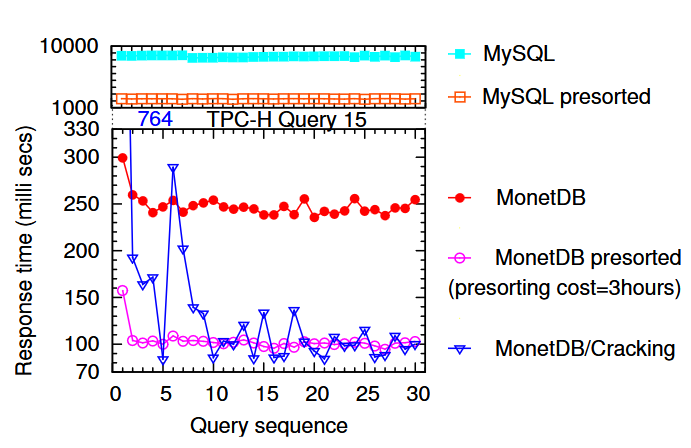
\includegraphics[width=250pt]{ressource/perf_comparaison.png}
    \caption{Notre objectif est de comparer avec ce genre de graphique notre implémentation et ce qui a déjà été fait.}
	\end{figure}
\end{frame}

\subsection{Où nous en sommes}
\begin{frame}
    \frametitle{Où nous en sommes}
 \begin{block}{Ce que nous avons implémenté}
    \begin{itemize}
        \item  Une BDD fonctionnelle pour la plupart des requêtes
        \item  Des optimisations du plan
        \item  Tester un grand nombre de requêtes et enregistrer les temps
    \end{itemize}
    \end{block}
    \begin{block}{Ce qu'il nous reste à faire}
    \begin{itemize}
        \item  Les optimisations mémoire
        \item  Comparer avec des implémentation existentes
        \item  Améliorer et optimiser certaines parties imparfaite de l'implémentation
    \end{itemize}
    \end{block}
\end{frame}

\section{But de notre TIPE}

\subsection{Description du jeux de données}

\begin{frame}
    \frametitle{Description du jeux de données} 

  \begin{block}{Nous avons choisi de travailler sur les données de wikipedia}
    \begin{itemize}
        \item  Des données de pages: titre, contenu, thème, modifications
        \item  Des données d'utilisateur: nom, date d'inscription, nombre de modification
        \item  Des révisions de pages
    \end{itemize}
    \end{block}
 \begin{block}{Des exemples de requêtes seraient}
    \begin{itemize}
        \item  Donner un classement des utilisateurs les plus actifs par catégorie
        \item  Utilisateurs experts d'une catégories
        \item  Pages les plus modifiées par catégories
    \end{itemize}
    \end{block}

\end{frame}


\subsection{Que faire des résultats ?}

\begin{frame}
    \frametitle{Que faire des résultats ?}

  \begin{block}{Nous avons plusieurs manières d'utiliser les résultats}
    \begin{itemize}
        \item  Récolter et afficher des statistiques utilisateur
        \item  Trier, comparer, selectionner
        \item  Recommander/Rechercher des pages selon des critères
    \end{itemize}
    \end{block}
\end{frame}


\section{Optimisations mémoire}

\subsection{Paradigme ligne VS colonne}

\begin{frame}
    \frametitle{Paradigme ligne VS colonne}
 \begin{figure}[h]
        \centering
        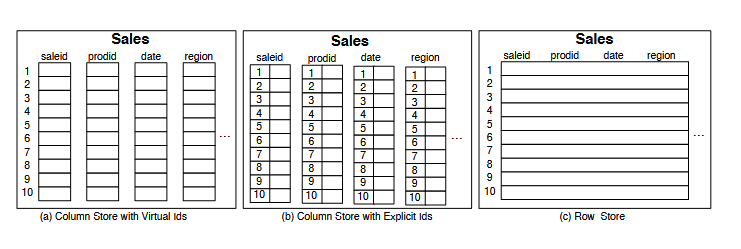
\includegraphics[width=300pt]{ressource/row_vs_column.png}
        \caption{Rendu physique des BDD orientées colonnes et BDD orientées lignes}
    \end{figure}
\end{frame}

\subsection{Indexation des données}

\begin{frame}
    \frametitle{Indexation des données}

\begin{figure}[h]
		\centering
		\includegraphics[width=250pt]{ressource/indexing.jpg}
    \caption{Un exemple de mise en oeuvre de l'indexation}
	\end{figure}

\end{frame}

\subsection{Fragmentation des données}

\begin{frame}
    \frametitle{Fragmentation des données}

	\begin{figure}[h]
		\centering
		\includegraphics[width=250pt]{ressource/cracking.png}
    \caption{Un exemple de mise en oeuvre du cracking}
	\end{figure}
\end{frame}

\section{Conclusion}
\subsection{Conclusion}
\begin{frame}
    \frametitle{Résumé}
    \begin{itemize}
        \item Les bases des Systèmes de Gestion de Base de Données
        \item Différentes optimisations naïve utilisant l'algèbre relationnelle
        \item Certaines optimisations dépendantes des données que notre SGBD possède
        \item Une analyse des résultats obtenus
    \end{itemize}
\end{frame}

\subsection{Nos ressources}
\begin{frame}
    \frametitle{Nos ressources}
    \textbf{Nos ressources:}
    \begin{itemize}
        \item \href{https://drive.google.com/file/d/1KNmuRBf8CV-s-zqdkUEP8iyYlPgFiglb/view?usp=drive_link}{\textit{The Design and Implementation of Modern Column-Oriented Database Systems} \(2013\)}
        \item \href{https://web.stanford.edu/class/cs345d-01/rl/cstore.pdf}{\textit{C-Store: A Column-oriented DBMS} \(2005\)}
        \item \href{https://link.springer.com/content/pdf/10.1007/s41019-020-00149-7.pdf}{\textit{A Survey on Advancing the DBMS Query Optimizer: Cardinality Estimation, Cost Model, and Plan Enumeration} \(2021\)}
        \item \href{https://www.microsoft.com/en-us/research/wp-content/uploads/2024/12/Extensible-Query-Optimizers-in-Practice.pdf}{\textit{Extensible Query Optimizers in Practice} \(2024\)}
        \item \href{http://webdam.inria.fr/Alice/}{\textit{Foundation of Databases} \(1995\)}
    \end{itemize}
\end{frame}

\end{document}

